\begin{figure}
    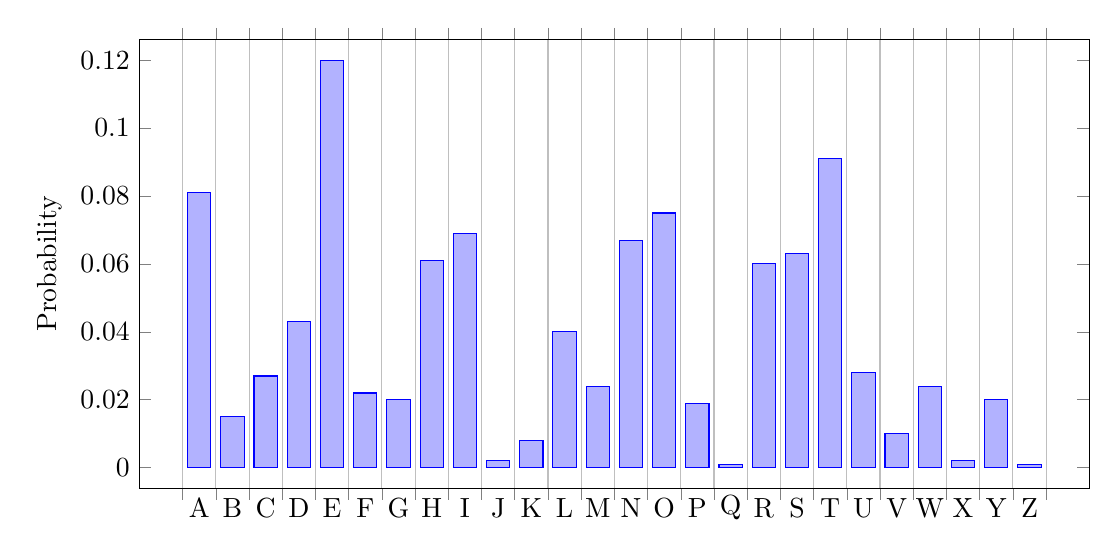
\begin{tikzpicture}
        \begin{axis}[
            ybar interval=0.7,
            symbolic x coords={A, B, C, D, E, F, G, H, I, J, K, L, M, N, O, P, Q, R, S, T, U, V, W, X, Y, Z, dummy},
            xtick=data,
            ylabel=Probability,
            restrict y to domain=0:0.12, % Ensures small values still show
            ymin=0,
            ymax=0.12,
            enlargelimits=0.05,
            yticklabel style={/pgf/number format/fixed, /pgf/number format/precision=2},
            every node near coord/.append style={font=\tiny}, % Prevents label overlap
            x tick label style={anchor=center, yshift=-3pt}, % Centers labels under bars
            x = 12pt,
        ]
        \addplot coordinates {
            (A,0.081) (B,0.015) (C,0.027) (D,0.043) (E,0.120)
            (F,0.022) (G,0.020) (H,0.061) (I,0.069) (J,0.002)
            (K,0.008) (L,0.040) (M,0.024) (N,0.067) (O,0.075)
            (P,0.019) (Q,0.001) (R,0.060) (S,0.063) (T,0.091)
            (U,0.028) (V,0.010) (W,0.024) (X,0.002) (Y,0.020) 
            (Z,0.001) (dummy,0.001)
        };
        
        \end{axis}
    \end{tikzpicture}
    \label{fig:letter_frequencies}
    \caption{relative Buchstabenhäufigkeiten der englischen Sprache}
\end{figure}